\documentclass[aspectratio=1610]{beamer}
 
%%%
%%% Copyright 2015 Christopher L. Phan
%%% 
%%% This work is licensed under a 
%%% Creative Commons Attribution-ShareAlike 4.0 
%%% International License.
%%%
%%% A copy of the license is available here:
%%% http://creativecommons.org/licenses/by-sa/4.0/
%%% 

%% packages
\usepackage{sagetex}
\usepackage{amsmath}
\usepackage{tikz}

\newcommand\copyrightnotice{\vfill {\tiny \textcolor{gray}{Copyright
2015 Christopher L.~Phan. This work is licensed under a 
\href{http://creativecommons.org/licenses/by-sa/4.0/}
{Creative Commons Attribution-ShareAlike 4.0 International License.}}}}

\begin{document}

\begin{frame}[fragile]
\frametitle{Derivative loop}

\begin{sagesilent}
save(plot(sin(x), x, -2*pi, 2*pi, figsize=[3, 2]), "deriv_loop_sin.pdf")
save(plot(cos(x), x, -2*pi, 2*pi, figsize=[3, 2]), "deriv_loop_cos.pdf")
save(plot(-sin(x), x, -2*pi, 2*pi, figsize=[3, 2]), "deriv_loop_-sin.pdf")
save(plot(-cos(x), x, -2*pi, 2*pi, figsize=[3, 2]), "deriv_loop_-cos.pdf")
\end{sagesilent}
\begin{center}
\begin{tikzpicture}
\node[inner sep=5pt] (sinecurve) at (0,0) 
{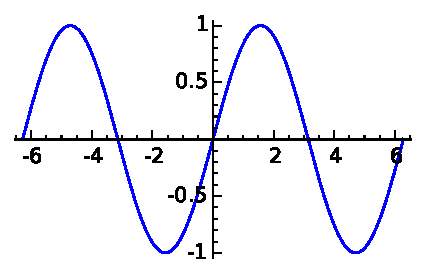
\includegraphics[width=.25\textwidth]{deriv_loop_sin.pdf}} ;

\node[anchor=south] at (sinecurve.north) {$\sin \theta$};

\node[inner sep=5pt] (cosinecurve) at (7,0) 
{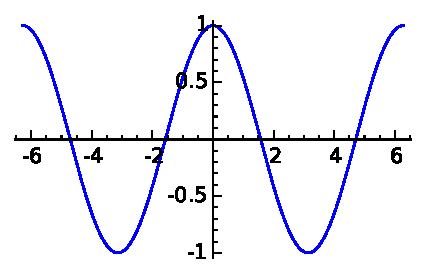
\includegraphics[width=.25\textwidth]{deriv_loop_cos.pdf}};

\node[anchor=south] at (cosinecurve.north) {$\cos \theta$};

\node[inner sep=5pt] (negsinecurve) at (7,-4) 
{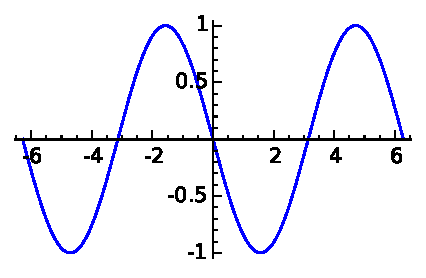
\includegraphics[width=.25\textwidth]{deriv_loop_-sin.pdf}};

\node[anchor=north] at (negsinecurve.south) {$-\sin \theta$};

\node[inner sep=5pt] (negcosinecurve) at (0,-4) 
{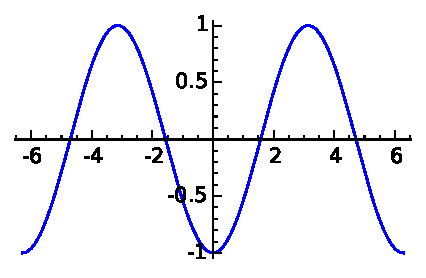
\includegraphics[width=.25\textwidth]{deriv_loop_-cos.pdf}};

\node[anchor=north] at (negcosinecurve.south) {$-\cos \theta$};


\draw[->,thick, purple] (sinecurve.east) -- (cosinecurve.west) node[anchor=south, midway] 
{$\displaystyle \frac{d}{d\theta}$};

\draw[->,thick, purple] (cosinecurve.south) -- (negsinecurve.north) node[anchor=west, midway] 
{$\displaystyle \frac{d}{d\theta}$};

\draw[->,thick, purple] (negsinecurve.west) -- (negcosinecurve.east) node[anchor=north, midway] 
{$\displaystyle \frac{d}{d\theta}$};

\draw[->,thick, purple] (negcosinecurve.north) -- (sinecurve.south) node[anchor=east, midway] 
{$\displaystyle \frac{d}{d\theta}$};

\end{tikzpicture}
\end{center}


\copyrightnotice

\end{frame}

\end{document}